% 被験者実験によってtransparencyを評価した
We evaluated the transparency, or inaudibility for human, of watermarks by a subjective experiment.
In this experiment, five participants are asked to listen to recorded sounds with embedded watermarks from a headphone and push a button when they notice unnatural noise.
For every participant, the output volume was set a constant value that he/she usually uses to listen to a music.
After that, the number of noticed watermarks is counted for each participant and sound.
We regarded a watermark to be noticed if a participant pushed the button within a second after the watermark is played.
% 4つの環境で録音された
Same as the experiments mentioned above, we tested the transparency in four environmental situations respectively to see the change of results depending on situations.
% elimination掛けたり掛けなかったり
In order to evaluate the effect of our watermark deletion program, we prepared two recordings for each situation, one is applied watermark deletion and the other is not.
In total, we used eight recordings in this experiment.
% 音源の情報
Each recording is one minute long and contains ten watermarks with 16 bytes payloads at randomly selected positions.

% 結果
\begin{figure}[htbp]
 \begin{center}
  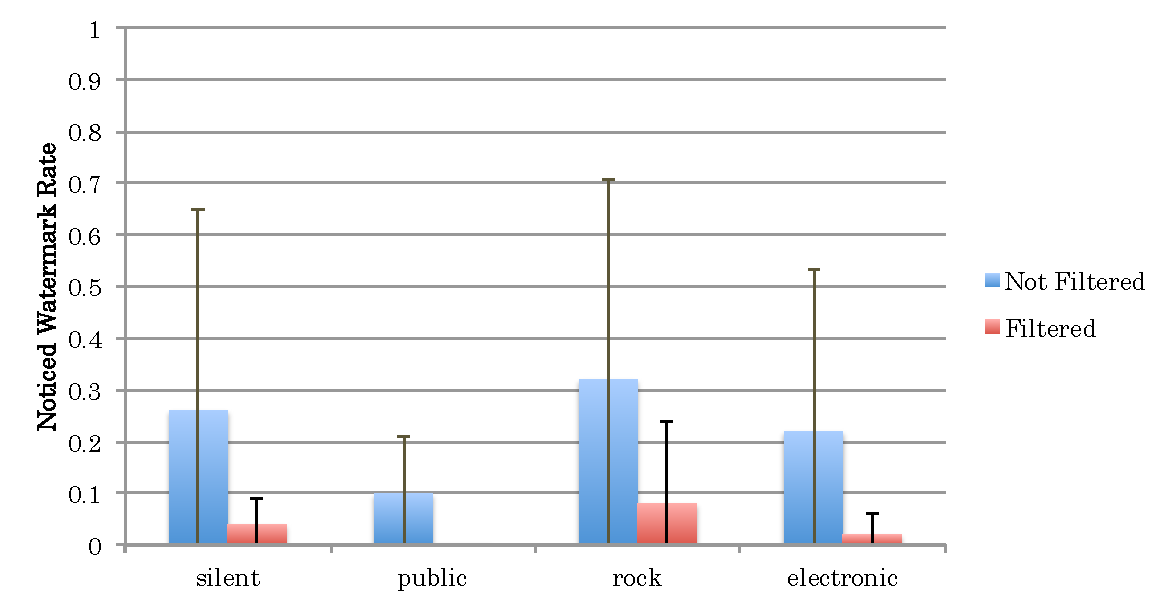
\includegraphics[width=120mm]{evaluation_transparency.pdf}
 \end{center}
 \caption{Mean rates of noticed watermarks for each conditions.}
 \label{fig:eval_tran}
\end{figure}

The result is shown in the graph above.
% notice rateはwatermark elimination以前からたかだか3割程度であって、
% 音源のqualityに大きな影響を与えていないと考えられる
Noticed watermark rates were at most 30 \% before being applied a watermark deletion in every situation.
% watermark eliminationを施した後では、ほとんど全く検知が不可能になっており、有効性が確認できる
After the deletion, the rates were much less than the source signals, and watermarks are virtually transparent.
These facts might indicate that our watermarking method can be used without decaying quality of sound.
% また、notice rateには個人差が大きく、特に年齢が高い被験者はほとんど検知することが出来なかったが、これはよく知られた聴覚の衰えによるものであろう
Interestingly, the difference of noticed watermark rates between individuals is very large, and young participants tend to notice more watermarks than mature ones.
This may be due to the universal high frequency hearing loss accompanied by aging.